% \documentclass[a4paper,10pt]{article}
% \usepackage[utf8]{inputenc}
% \usepackage{geometry}
% \usepackage[table]{xcolor}
% \usepackage{colortbl}
% \usepackage{color,soul}
% \geometry{margin=0.8in}
% \usepackage{xcolor}
% \usepackage{tikz}
% \usepackage{minted}
% \definecolor{bgcolor}{rgb}{0.8, 0.9, 0.5} % 
% \definecolor{bgcolor1}{rgb}{0.95, 0.95, 0.95} % Light Gray
% \definecolor{bgcolor2}{rgb}{0.85, 0.92, 1.0}  % Soft Blue
% \definecolor{bgcolor3}{rgb}{0.9, 0.85, 1.0}   % Light Purple
% \definecolor{bgcolor4}{rgb}{0.95, 0.88, 0.76} % Warm Beige
% \definecolor{bgcolor5}{rgb}{0.8, 0.95, 0.8}   % Gentle Green
% \definecolor{bgcolor6}{rgb}{1.0, 0.87, 0.87}  % Pastel Red
% \definecolor{bgcolor7}{rgb}{0.86, 0.93, 0.83} % Mint Green
% \definecolor{bgcolor8}{rgb}{0.98, 0.85, 0.94} % Soft Pink
% \definecolor{bgcolor9}{rgb}{0.87, 0.94, 0.98} % Sky Blue
% \definecolor{bgcolor10}{rgb}{0.96, 0.96, 0.82} % Pale Yellow
% 
% \begin{document}
\section*{Array Problem Solutions}

\noindent\textbf{Problem: Equilibrium Index of Array}
\begin{minted}[
    bgcolor=bgcolor1,
    frame=lines,
    framesep=5mm,
    rulecolor=\color{black},
    linenos,
    numbersep=5pt,
    fontsize=\normalsize
]{python}
def equilibrium_index(nums: List[int]) -> int:
    """
    Finds an equilibrium index in an array.
    An equilibrium index is an index such that the sum of elements
    at lower indices is equal to the sum of elements at higher indices.
    Time Complexity: O(n), Space: O(1)
    """
    total_sum = sum(nums)
    left_sum = 0
    for i in range(len(nums)):
        right_sum = total_sum - left_sum - nums[i]
        if left_sum == right_sum:
            return i
        left_sum += nums[i]
    return -1 # No equilibrium index found
\end{minted}

\noindent\textbf{Problem: Largest Sum Subarray (Kadane’s)}
\begin{minted}[
    bgcolor=bgcolor2,
    frame=lines,
    framesep=5mm,
    rulecolor=\color{black},
    linenos,
    numbersep=5pt,
    fontsize=\normalsize
]{python}
def largest_sum_subarray(nums: List[int]) -> int:
    """
    Finds the maximum sum of a contiguous subarray using Kadane's algorithm.
    Time Complexity: O(n), Space: O(1)
    """
    if not nums:
        return 0 # Or handle as per problem statement for empty array

    max_so_far = nums[0]
    current_max = nums[0]

    for i in range(1, len(nums)):
        current_max = max(nums[i], current_max + nums[i]) 
        max_so_far = max(max_so_far, current_max)
    
    return max_so_far
\end{minted}

\noindent\textbf{Problem: Merge Two Sorted Arrays}
\begin{minted}[
    bgcolor=bgcolor3,
    frame=lines,
    framesep=5mm,
    rulecolor=\color{black},
    linenos,
    numbersep=5pt,
    fontsize=\normalsize
]{python}
def merge_two_sorted_arrays(nums1: List[int], nums2: List[int]) -> List[int]:
    """
    Merges two sorted arrays into a single sorted array using a two-pointer technique.
    Time Complexity: O(n + m), Space: O(n + m) (for the new merged array)
    """
    m, n = len(nums1), len(nums2)
    merged_array =  * (m + n)
    p1, p2, p_merged = 0, 0, 0

    while p1 < m and p2 < n:
        if nums1[p1] < nums2[p2]:
            merged_array[p_merged] = nums1[p1]
            p1 += 1
        else:
            merged_array[p_merged] = nums2[p2]
            p2 += 1
        p_merged += 1
    
    # Append any remaining elements from nums1
    while p1 < m:
        merged_array[p_merged] = nums1[p1]
        p1 += 1
        p_merged += 1
    
    # Append any remaining elements from nums2
    while p2 < n:
        merged_array[p_merged] = nums2[p2]
        p2 += 1
        p_merged += 1
    
    return merged_array
    # if space is contraint put at back of one array apply algo from back to front
\end{minted}

\noindent\textbf{Problem: Move Zeroes}
\begin{minted}[
    bgcolor=bgcolor4,
    frame=lines,
    framesep=5mm,
    rulecolor=\color{black},
    linenos,
    numbersep=5pt,
    fontsize=\normalsize
]{python}
def move_zeroes(nums: List[int]) -> None:
    """
    Move all zeros to end, preserving order of non-zero elements.
    This uses a two-pointer technique to swap non-zero elements forward.
    Time Complexity: O(n), Space: O(1)
    """
    j = 0 # Pointer for the next non-zero element to be placed
    for i in range(len(nums)): # Pointer to iterate through the array
        if nums[i] != 0:
            # If the current element is non-zero, swap it with the element at j
            # and increment j. This places non-zero elements at the front
            # while maintaining their relative order.
            nums[j], nums[i] = nums[i], nums[j]
            j += 1
\end{minted}

\noindent\textbf{Problem: Left Rotate Array by D Places}
\begin{minted}[
    bgcolor=bgcolor5,
    frame=lines,
    framesep=5mm,
    rulecolor=\color{black},
    linenos,
    numbersep=5pt,
    fontsize=\normalsize
]{python}
def _reverse_subarray(nums: List[int], start: int, end: int) -> None:
    """Helper function to reverse a subarray in-place."""
    while start < end:
        nums[start], nums[end] = nums[end], nums[start]
        start += 1
        end -= 1

def left_rotate_array_by_d_places(nums: List[int], d: int) -> None:
    """
    Left rotates an array by D places using the reversal algorithm. [3]
    Time Complexity: O(n), Space: O(1)
    """
    n = len(nums)
    if n == 0:
        return
    
    d = d % n # Handle cases where d >= n [3]

    if d == 0: # No rotation needed
        return

    # Reverse the first d elements (0 to d-1)
    _reverse_subarray(nums, 0, d - 1)
    # Reverse the remaining n-d elements (d to n-1)
    _reverse_subarray(nums, d, n - 1)
    # Reverse the entire array (0 to n-1)
    _reverse_subarray(nums, 0, n - 1)
\end{minted}

\noindent\textbf{Problem: Leaders in an Array}
\begin{minted}[
    bgcolor=bgcolor6,
    frame=lines,
    framesep=5mm,
    rulecolor=\color{black},
    linenos,
    numbersep=5pt,
    fontsize=\normalsize
]{python}
def find_leaders_in_array(nums: List[int]) -> List[int]:
    """
    Finds all leaders in an array. A leader is an element that is greater
    than or equal to all the elements to its right. The rightmost element is
    always a leader.
    Time Complexity: O(n), Space: O(1) (excluding the result list)
    """
    if not nums:
        return []
    
    n = len(nums)
    leaders = []
    max_right = nums[n - 1] # The rightmost element is always a leader [3]
    leaders.append(max_right)

    # Traverse from right to left [3]
    for i in range(n - 2, -1, -1):
        if nums[i] >= max_right:
            max_right = nums[i]
            leaders.append(max_right)
    
    # Leaders are typically expected in order of appearance in array,
    # so reverse the list if built from right-to-left.
    return leaders[::-1]
\end{minted}

\noindent\textbf{Problem: Maximum Difference with Order}
\begin{minted}[
    bgcolor=bgcolor7,
    frame=lines,
    framesep=5mm,
    rulecolor=\color{black},
    linenos,
    numbersep=5pt,
    fontsize=\normalsize
]{python}
def max_difference_with_order(prices: List[int]) -> int:
    """
    Finds the maximum difference between two elements in an array such that
    the smaller element appears before the larger element (i.e., buy low, sell high).
    It tracks the minimum element seen so far.
    Time Complexity: O(n), Space: O(1)
    """
    if len(prices) < 2:
        return 0 # Return 0 or -1 based on problem requirement for no profit. [3]

    min_price_so_far = prices
    max_profit = 0

    for i in range(1, len(prices)):
        max_profit = max(max_profit, prices[i] - min_price_so_far)
        min_price_so_far = min(min_price_so_far, prices[i])
    
    return max_profit
\end{minted}

\noindent\textbf{Problem: Frequencies in Sorted Array}
\begin{minted}[
    bgcolor=bgcolor8,
    frame=lines,
    framesep=5mm,
    rulecolor=\color{black},
    linenos,
    numbersep=5pt,
    fontsize=\normalsize
]{python}
from typing import List, Tuple

def frequencies_in_sorted_array(nums: List[int]) -> List[Tuple[int, int]]:
    """
    Calculates the frequency of each element in a sorted array by traversing
    and counting frequency changes.
    Time Complexity: O(n), Space: O(1) (excluding the result list)
    """
    if not nums:
        return []
    
    frequencies = []
    n = len(nums)
    count = 1
    
    for i in range(1, n):
        if nums[i] == nums[i-1]:
            count += 1
        else:
            frequencies.append((nums[i-1], count))
            count = 1
    
    # Add the last element's frequency
    frequencies.append((nums[n-1], count))
    
    return frequencies
\end{minted}

\noindent\textbf{Problem: Stock Buy and Sell (Multiple Transactions)}
\begin{minted}[
    bgcolor=bgcolor9,
    frame=lines,
    framesep=5mm,
    rulecolor=\color{black},
    linenos,
    numbersep=5pt,
    fontsize=\normalsize
]{python}
def stock_buy_and_sell(prices: List[int]) -> int:
    """
    Calculates the maximum profit from buying and selling stocks,
    allowing multiple transactions. This is done by tracking ascending subarrays for profit.
    Time Complexity: O(n), Space: O(1)
    """
    if len(prices) < 2:
        return 0
    
    max_profit = 0
    for i in range(1, len(prices)):
        # If today's price is higher than yesterday's, we can make a profit by
        # buying yesterday and selling today. Add this profit.
        if prices[i] > prices[i-1]:
            max_profit += prices[i] - prices[i-1]
            
    return max_profit
\end{minted}

\noindent\textbf{Problem: Maximum Circular Subarray Sum}
\begin{minted}[
    bgcolor=bgcolor10,
    frame=lines,
    framesep=5mm,
    rulecolor=\color{black},
    linenos,
    numbersep=5pt,
    fontsize=\normalsize
]{python}
def max_circular_subarray_sum(nums: List[int]) -> int:
    """
    Finds the maximum possible sum of a non-empty subarray of a circular array.
    Kadane's for non-wrapping sums and total_sum - min_subarray_sum for wrapping sums.
    Time Complexity: O(n), Space: O(1)
    """
    if not nums:
        return 0

    # Case 1: Max sum subarray is non-wrapping (standard Kadane's)
    max_straight_sum = nums[0]
    current_max = nums[0]
    for i in range(1, len(nums)):
        current_max = max(nums[i], current_max + nums[i])
        max_straight_sum = max(max_straight_sum, current_max)
    
    # Case 2: Max sum subarray is wrapping (total sum - min sum non-wrapping subarray)
    total_sum = sum(nums)
    
    min_straight_sum = nums[0]
    current_min = nums[0]
    for i in range(1, len(nums)):
        current_min = min(nums[i], current_min + nums[i])
        min_straight_sum = min(min_straight_sum, current_min)
    
    # Edge case: If all numbers are negative, max_straight_sum will be the largest negative number.
    # In this scenario, total_sum - min_straight_sum would result in 0 or a positive value,
    # which is incorrect as an empty subarray is not allowed.
    if total_sum == min_straight_sum: # Implies all elements are negative or zero (e.g., [-1, -2])
        return max_straight_sum # Only the non-wrapping case is valid
    
    max_wrapping_sum = total_sum - min_straight_sum
    
    return max(max_straight_sum, max_wrapping_sum)
\end{minted}

\noindent\textbf{Problem: Majority Element (Boyer-Moore Voting Algorithm)}
\begin{minted}[
    bgcolor=bgcolor1,
    frame=lines,
    framesep=5mm,
    rulecolor=\color{black},
    linenos,
    numbersep=5pt,
    fontsize=\normalsize
]{python}
def majority_element_boyer_moore(nums: List[int]) -> int:
    """
    Finds the majority element in an array using Boyer-Moore Voting Algorithm. 
    The majority element appears more than n/2 times.
    Time Complexity: O(n), Space: O(1)
    """
    candidate = None
    count = 0

    for num in nums:
        if count == 0:
            candidate = num
            count = 1
        elif num == candidate:
            count += 1
        else:
            count -= 1
            
    # The Boyer-Moore algorithm guarantees that if a majority element exists,
    # it will be the candidate. If the problem guarantees a majority element,
    # no second pass verification is needed. If not, a verification step
    # (counting occurrences of candidate) would be required.
    
    return candidate
\end{minted}

\noindent\textbf{Problem: Trapping Rain Water}
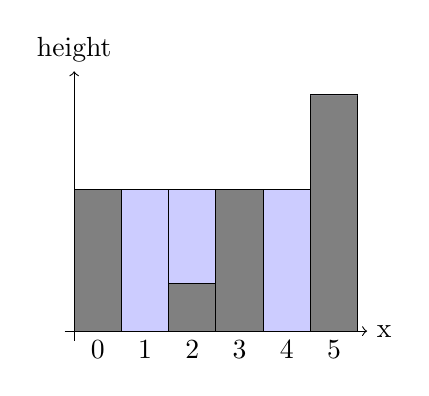
\begin{tikzpicture}[scale=0.6]
  % Data: index/height/water
  \foreach \i/\h/\w in {
    0/3/0,
    1/0/3,
    2/1/2,
    3/3/0,
    4/0/3,
    5/5/0} {
    % draw bar
    \draw[fill=black!50] (\i,0) rectangle ++(1,\h);
    % draw water (height \w) on top of bar
    \draw[fill=blue!20] (\i,\h) rectangle ++(1,\w);
  }
  % axes
  \draw[->] (-0.2,0) -- (6.2,0) node[right] {x};
  \draw[->] (0,-0.2) -- (0,5.5) node[above] {height};
  % x labels
  \foreach \i in {0,...,5}
    \node[below] at (\i+0.5,0) {\i};
\end{tikzpicture}

\begin{minted}[
    bgcolor=bgcolor2,
    frame=lines,
    framesep=5mm,
    rulecolor=\color{black},
    linenos,
    numbersep=5pt,
    fontsize=\normalsize
]{python}
def trap_rain_water(height: List[int]) -> int:
    """
    Calculates the amount of rain water that can be trapped between bars.
    Uses a two-pointer approach which is space-efficient.
    Time Complexity: O(n), Space: O(1)
    """    
    # If fewer than 3 bars, no “bucket” can form see pic for clarity water stored over bar
    if not height or len(height) < 3:
        return 0
    left, right = 0, len(height) - 1
    left_max, right_max = 0, 0
    water_trapped = 0

    while left < right:
        if height[left] < height[right]:
            # Water level determined by left side, move left pointer
            if height[left] >= left_max:
                left_max = height[left]
            else:
                water_trapped += left_max - height[left]
            left += 1
        else:
            # Water level determined by right side, move right pointer
            if height[right] >= right_max:
                right_max = height[right]
            else:
                water_trapped += right_max - height[right]
            right -= 1
            
    return water_trapped
\end{minted}

\noindent\textbf{Problem: Minimum Consecutive Flips}
\begin{minted}[
    bgcolor=bgcolor3,
    frame=lines,
    framesep=5mm,
    rulecolor=\color{black},
    linenos,
    numbersep=5pt,
    fontsize=\normalsize
]{python}
def min_consecutive_flips(binary_array: List[int]) -> int:
    """
    Finds the minimum number of flips needed to make all elements in a
    binary array the same (all 0s or all 1s). A flip changes a contiguous block.
    This is achieved by counting alternating groups and choosing the minimum.
    Time Complexity: O(n), Space: O(1)
    """
    if not binary_array:
        return 0
    
    num_zeros_blocks = 0
    num_ones_blocks = 0

    # Initialize counts for the first block
    if binary_array[0] == 0:
        num_zeros_blocks = 1
    else:
        num_ones_blocks = 1

    # Iterate through the array to find transitions and count blocks
    for i in range(1, len(binary_array)):
        if binary_array[i] != binary_array[i-1]:
            if binary_array[i] == 0:
                num_zeros_blocks += 1
            else:
                num_ones_blocks += 1
    
    # The minimum flips required is the smaller count of blocks.
    # For example, if you have '0011100', blocks are (00, 111, 00).
    # Zero blocks: 2. One blocks: 1. Min is 1 (flip '111' to make all 0s).
    return min(num_zeros_blocks, num_ones_blocks)
\end{minted}

\noindent\textbf{Problem: Sliding Window Technique (Example: Max Sum Subarray of Size K)}
\begin{minted}[
    bgcolor=bgcolor4,
    frame=lines,
    framesep=5mm,
    rulecolor=\color{black},
    linenos,
    numbersep=5pt,
    fontsize=\normalsize
]{python}
def max_sum_subarray_of_size_k(nums: List[int], k: int) -> int:
    """
    Finds the maximum sum of a subarray of a fixed size K using the sliding window technique. [5]
    Time Complexity: O(n), Space: O(1)
    """
    if k <= 0 or not nums or k > len(nums):
        return 0 # Or raise error, based on problem specific constraints
    
    current_window_sum = 0
    
    # Calculate sum of the first window (size k)
    for i in range(k):
        current_window_sum += nums[i]
    
    max_window_sum = current_window_sum
    
    # Slide the window across the array
    for i in range(k, len(nums)):
        current_window_sum += nums[i] - nums[i - k] # Add new element, subtract old element
        max_window_sum = max(max_window_sum, current_window_sum)
        
    return max_window_sum
\end{minted}

\noindent\textbf{Problem: Consecutive Ones III (Max Consecutive Ones with K Flips)}
\begin{minted}[
    bgcolor=bgcolor5,
    frame=lines,
    framesep=5mm,
    rulecolor=\color{black},
    linenos,
    numbersep=5pt,
    fontsize=\normalsize
]{python}
def longest_ones(nums: List[int], k: int) -> int:
    """
    Given a binary array nums and an integer k, return the maximum number of
    consecutive 1's in the array if you can flip at most k 0's.
    This uses a sliding window where the window expands and shrinks based on zero count.
    Time Complexity: O(n) 2*n traversal by right and left , Space: O(1)
    """
    left = 0
    zero_count = 0
    max_length = 0

    for right in range(len(nums)):
        if nums[right] == 0:
            zero_count += 1
        
        # If zero_count exceeds k, shrink the window from the left by moving 'left' pointer
        while zero_count > k:
            if nums[left] == 0: # If the element leaving the window is a zero, decrement zero_count
                zero_count -= 1
            left += 1
        
        # Update max_length for the current valid window
        max_length = max(max_length, right - left + 1)
        
    return max_length
\end{minted}
\noindent\textbf{Problem: Max Consecutive Ones with K Flips (Strictly single traversal) }
\begin{minted}[
    bgcolor=bgcolor5,
    frame=lines,
    framesep=5mm,
    rulecolor=\color{black},
    linenos,
    numbersep=5pt,
    fontsize=\normalsize
]{python}
def longest_ones(nums: List[int], k: int) -> int:
    """
    Given a binary array nums and an integer k, return the maximum number of
    consecutive 1's in the array if you can flip at most k 0's.
    This uses a sliding window where the window expands and shrinks based on zero count. 
    Time Complexity: O(n) Strictly single traversal , Space: O(1)
    """
    left ,zc ,max_len = 0 ,0 ,0
      for right in range(len(nums)):
        # 1) Expand window to include nums[right]
        if nums[right] == 0:
            zc += 1

        # 2) If too many zeros, shrink from the left until zc <= k
        if zc > k:
            # If the element at `left` was a flipped‐zero, un‐flip it
            if nums[left] == 0:
                zc -= 1
            left += 1

        # 3) Now window [left..right] has <= k zeros: record its size
        #    We only update when it's valid; this guarantees max_len always
        #    reflects a window we could actually achieve by flipping <= k zeros.
        if zc <= k:
            max_len = max(max_len, right - left + 1)

    return max_len

\end{minted}
\noindent\textbf{Problem: Longest Substring with At Most K Distinct Characters}
\begin{minted}[
    bgcolor=bgcolor6,
    frame=lines,
    framesep=5mm,
    rulecolor=\color{black},
    linenos,
    numbersep=5pt,
    fontsize=\normalsize
]{python}


def longest_substring_k_distinct(s: str, k: int) -> int:
    """
    Finds the length of the longest substring with at most K distinct characters.
    This is analogous to the "Fruit in Basket" problem. 
    Uses a sliding window with a hash map for frequency tracking. 
    Time Complexity: O(n), Space: O(k) (for the frequency map, max k distinct chars)
    """
    if k == 0:
        return 0
    
    char_freq: Dict[str, int] = {}
    left = 0
    max_length = 0

    for right in range(len(s)):
        char_freq[s[right]] = char_freq.get(s[right], 0) + 1
        
        # Shrink the window from the left if distinct characters exceed k
        while len(char_freq) > k:
            char_freq[s[left]] -= 1
            if char_freq[s[left]] == 0: # If count becomes 0, remove char from map
                del char_freq[s[left]]
            left += 1
        
        # Update max_length for the current valid window
        max_length = max(max_length, right - left + 1)
        
    return max_length

    # Can easily converted it to above strictly O(N) by replacing while with if
    #And checking the size of map before updating max_length .!Just this much


    ###########################ALTERNATE IMPLEMENTATION########################

def longest_substring_k_distinct(s: str, k: int) -> int:
    """
    Longest substring with at most k distinct characters.
    Time: O(n), Space: O(k)
    """
    if k == 0 or not s:
        return 0

    left = 0
    max_len = 0
    # char → last index seen; insertion order = window order
    window: "OrderedDict[str,int]" = OrderedDict()

    for right, ch in enumerate(s):
        # If ch already in window, delete+reinsert to update its “recentness”
        if ch in window:
            del window[ch]
        window[ch] = right

        # If we now have > k distinct, evict the oldest:
        if len(window) > k:
            # popitem(last=False) removes the first key inserted
            old_char, old_index = window.popitem(last=False)
            # move left pointer just beyond that char’s last occurrence
            left = old_index + 1

        # window is valid: [left..right] contains <= k distinct characters
        max_len = max(max_len, right - left + 1)

    return max_len

\end{minted}

\noindent\textbf{Problem: Longest Substring Without Repeating Characters}
\begin{minted}[
    bgcolor=bgcolor7,
    frame=lines,
    framesep=5mm,
    rulecolor=\color{black},
    linenos,
    numbersep=5pt,
    fontsize=\normalsize
]{python}
def length_of_longest_substring(s: str) -> int:
    """
    Finds the length of the longest substring without repeating characters.
    Uses a sliding window with a map to track the last seen index of characters. 
    Time Complexity: O(n), Space: O(alphabet_size) (for the character index map)
    """
    char_index_map: Dict[str, int] = {} # Stores char -> its last seen index
    left = 0
    max_length = 0

    for right in range(len(s)):
        current_char = s[right]
        
        # If current_char is already in the map AND its last seen index
        # is within the current window (i.e., char_index_map[current_char] >= left),
        # then move the left pointer to avoid the repeating character.
        if current_char in char_index_map and char_index_map[current_char] >= left:
            left = char_index_map[current_char] + 1
        
        char_index_map[current_char] = right # Update last seen index of current_char
        max_length = max(max_length, right - left + 1)
        
    return max_length
\end{minted}

\noindent\textbf{Problem: Sub array sum = K for array containing positives, zero and negatives}
\begin{minted}[
    bgcolor=bgcolor8,
    frame=lines,
    framesep=5mm,
    rulecolor=\color{black},
    linenos,
    numbersep=5pt,
    fontsize=\normalsize
]{python}
def subarray_sum_equals_k(nums: List[int], k: int) -> int:
    """
    Returns the number of contiguous subarrays whose sum == k.
    Handles negative numbers—sliding window won’t work here.
    Time: O(n), Space: O(n)
    """
    count = 0
    prefix_sum = 0
    # Map from prefix_sum value to how many times we've seen it so far.
    # We seed with {0:1} so that any prefix_sum == k at index i counts as a valid subarray [0..i].
    seen: Dict[int,int] = {0: 1}

    for x in nums:
        prefix_sum += x
        # If (prefix_sum - k) appeared before, those are subarrays ending here summing to k
        if (prefix_sum - k) in seen:
            count += seen[prefix_sum - k]

        # Record this prefix_sum for future subarrays
        seen[prefix_sum] = seen.get(prefix_sum, 0) + 1

    return count
    ####   Apply Same for Binary Subarray with sum S
\end{minted}
\noindent\textbf{Problem: Zero Containg subarray with sum K(Binary Subarray ) }
\begin{minted}[
    bgcolor=bgcolor8,
    frame=lines,
    framesep=5mm,
    rulecolor=\color{black},
    linenos,
    numbersep=5pt,
    fontsize=\normalsize
]{python}
def subarray_sum_equals_k(nums: List[int], k: int) -> int:
    """
    Returns the number of contiguous subarrays whose sum == k.
    This can't handle negatives!!!
    Time: O(n), Space: O(n)
    """
    def numSubarraysWithSum(nums, k):
        def atMost(s):
            if s < 0:
                return 0
            left = 0
            count = 0
            curr_sum = 0
            for right in range(len(nums)):
                curr_sum += nums[right]
                while curr_sum > s:
                    curr_sum -= nums[left]
                    left += 1
                count += right - left + 1
            return count

    return atMost(k) - atMost(k - 1)   
    ####   Apply Same for Binary Subarray with sum S
\end{minted}
\noindent\textbf{Problem: Count All Substrings With Exactly K Distinct Characters}
\begin{minted}[
    bgcolor=bgcolor9,
    frame=lines,
    framesep=5mm,
    rulecolor=\color{black},
    linenos,
    numbersep=5pt,
    fontsize=\normalsize
]{python}


def _at_most_k_distinct_substrings(s: str, k: int) -> int:
    """
    Helper function to count substrings with at most K distinct characters.
    Time Complexity: O(n), Space: O(alphabet_size)
    """
    if k < 0: # No substrings can have negative distinct characters
        return 0
    if k == 0: # Only empty string or no distinct characters, usually 0 substrings
        return 0

    char_freq: Dict[str, int] = {}
    left = 0
    count = 0

    for right in range(len(s)):
        char_freq[s[right]] = char_freq.get(s[right], 0) + 1
        
        while len(char_freq) > k:
            char_freq[s[left]] -= 1
            if char_freq[s[left]] == 0:
                del char_freq[s[left]]
            left += 1
        
        # All substrings ending at 'right' and starting from 'left' up to 'right'
        # have at most k distinct characters. The count is the length of the current window.
        count += (right - left + 1)
        
    return count

def count_exactly_k_distinct_substrings(s: str, k: int) -> int:
    """
    Counts the number of substrings with exactly K distinct characters.
    Uses the principle: count(exactly K) = count(at most K) - count(at most K-1). 
    Time Complexity: O(n), Space: O(alphabet_size)
    """
    return _at_most_k_distinct_substrings(s, k) - _at_most_k_distinct_substrings(s, k - 1)
    #Because using 2 pointers we cant take in account for abbbbbccdce k=3 
    #Lots of correct windows are skipped due to incrementing r for exact matching
\end{minted}

\noindent\textbf{Problem: Print All Substrings With Exactly K Distinct Characters}
\begin{minted}[
    bgcolor=bgcolor10,
    frame=lines,
    framesep=5mm,
    rulecolor=\color{black},
    linenos,
    numbersep=5pt,
    fontsize=\normalsize
]{python}
from typing import List, Dict

def print_exactly_k_distinct_substrings(s: str, k: int) -> List[str]:
    """
    Prints all substrings with exactly K distinct characters.
    It iterates through all possible start and end points of substrings. 
    Time Complexity: O(n^2 * alphabet_size) (due to nested loops and map operations)
    Space Complexity: O(alphabet_size) (for the frequency map)
    """
    result_substrings: List[str] = []
    n = len(s)

    for i in range(n): # Start of substring
        char_freq: Dict[str, int] = {}
        distinct_count = 0
        for j in range(i, n): # End of substring
            char = s[j]
            if char_freq.get(char, 0) == 0: # New distinct character found
                distinct_count += 1
            char_freq[char] = char_freq.get(char, 0) + 1
            
            if distinct_count == k:
                result_substrings.append(s[i:j+1])
            elif distinct_count > k:
                # Optimization: If distinct count exceeds k, no further substrings
                # starting at 'i' will have exactly k distinct characters by extending.
                break 
    return result_substrings
\end{minted}

\noindent\textbf{Problem: Prefix Sum Technique (Example: Range Sum Query)}
\begin{minted}[
    bgcolor=bgcolor1,
    frame=lines,
    framesep=5mm,
    rulecolor=\color{black},
    linenos,
    numbersep=5pt,
    fontsize=\normalsize
]{python}
class PrefixSumArray:
    """
    Implements the prefix sum technique for efficient range sum queries.
    Preprocessing Time Complexity: O(n)
    Query Time Complexity: O(1) [8]
    Space Complexity: O(n)
    """
    def __init__(self, nums: List[int]):
        # Build prefix sum array [7]
        self.prefix_sum =  * (len(nums) + 1)
        for i in range(len(nums)):
            self.prefix_sum[i+1] = self.prefix_sum[i] + nums[i]
            
    def query_range_sum(self, start_idx: int, end_idx: int) -> int:
        """
        Returns the sum of elements in the range [start_idx, end_idx] (inclusive).
        Assumes 0-based indexing for input array.
        """
        if not (0 <= start_idx <= end_idx < len(self.prefix_sum) - 1):
            raise IndexError("Invalid range indices")
        
        return self.prefix_sum[end_idx + 1] - self.prefix_sum[start_idx]
\end{minted}

\noindent\textbf{Problem: Maximum Appearing Element in Ranges (Line Sweep)}
\begin{minted}[
    bgcolor=bgcolor2,
    frame=lines,
    framesep=5mm,
    rulecolor=\color{black},
    linenos,
    numbersep=5pt,
    fontsize=\normalsize
]{python}
def max_appearing_element_in_ranges(L: List[int], R: List[int]) -> int:
    """
    Finds the element that appears maximum number of times across given ranges [L[i], R[i]].
    Uses a difference array and then computes prefix sums to find the maximum.
    Time Complexity: O(N + max_val), where N is number of ranges, max_val is max R[i].
    Space Complexity: O(max_val)
    """
    if not L or not R or len(L) != len(R):
        return -1 # Handle invalid input
    
    max_range_val = 0
    if R:
        max_range_val = max(R)

    # Create a difference array. Size max_range_val + 2 to handle R[i]+1.
    # If values can be very large, coordinate compression might be needed.
    freq_arr =  * (max_range_val + 2) 

    for i in range(len(L)):
        freq_arr[L[i]] += 1
        freq_arr[R[i] + 1] -= 1
    
    max_frequency = 0
    result_element = -1
    current_frequency = 0

    # Compute prefix sums on the difference array to get actual frequencies
    for i in range(max_range_val + 1):
        current_frequency += freq_arr[i]
        if current_frequency > max_frequency:
            max_frequency = current_frequency
            result_element = i
            
    return result_element
\end{minted}

\noindent\textbf{Problem: Subarray with Given Sum (Count)}
\begin{minted}[
    bgcolor=bgcolor3,
    frame=lines,
    framesep=5mm,
    rulecolor=\color{black},
    linenos,
    numbersep=5pt,
    fontsize=\normalsize
]{python}
def count_subarrays_with_sum_k(nums: List[int], k: int) -> int:
    """
    Count how many contiguous subarrays of a positive-only array sum exactly to k.
    Time: O(n), Space: O(1)
    """
    count = 0
    curr_sum = 0
    left = 0

    for right, v in enumerate(nums):
        # 1) Extend window to the right
        curr_sum += v

        # 2) Shrink from the left until sum <= k
        #    (valid because every element >= 0)
        while curr_sum > k and left <= right:
            curr_sum -= nums[left]
            left += 1

        # 3) If we hit exactly k, that window [left..right] is one match
        if curr_sum == k:
            count += 1

    return count
    # For calculating longest such similiar code. 
    ####################################################################################
def subarray_sum_count(nums: List[int], target_sum: int) -> int:
    """
    Counts the number of subarrays that sum up to a specific target_sum.
    Works for arrays with positive, negative, and zero integers using prefix sums and a hash map. 
    Time Complexity: O(n), Space: O(n) (for the prefix sum map)
    """
    # prefix_sums_freq: maps a prefix sum to its frequency
    prefix_sums_freq: Dict[int, int] = {0: 1} # Initialize with 0 sum occurring once (empty prefix)
    current_sum = 0
    count = 0

    for num in nums:
        current_sum += num
        # If (current_sum - target_sum) exists in the map,
        # it means there's a previous prefix sum that, when subtracted
        # from the current_sum, results in target_sum.
        count += prefix_sums_freq.get(current_sum - target_sum, 0)
        
        # Add the current_sum to the map, incrementing its frequency
        prefix_sums_freq[current_sum] = prefix_sums_freq.get(current_sum, 0) + 1
        
    return count
\end{minted}

\noindent\textbf{Problem: Next Permutation}
\begin{minted}[
    bgcolor=bgcolor4,
    frame=lines,
    framesep=5mm,
    rulecolor=\color{black},
    linenos,
    numbersep=5pt,
    fontsize=\normalsize
]{python}
def next_permutation(nums: List[int]) -> None:
    """
    Rearranges numbers into the lexicographically next greater permutation.
    It involves finding the longest non-increasing suffix, swapping a pivot, and reversing.
    Time Complexity: O(n), Space: O(1)
    """
    n = len(nums)
    
    # 1. Find the largest index k such that nums[k] < nums[k+1]
    # This identifies the "pivot" point to change the permutation.
    k = -1
    for i in range(n - 2, -1, -1):
        if nums[i] < nums[i+1]:
            k = i
            break
    
    if k == -1: # If no such index exists, the permutation is the last permutation
        nums.reverse() # In this case, reverse the entire array to get the first permutation.
        return

    # 2. Find the largest index l greater than k such that nums[k] < nums[l]
    # This finds the smallest element in the suffix that is greater than nums[k].
    l = -1
    for i in range(n - 1, k, -1):
        if nums[i] > nums[k]:
            l = i
            break
            
    # 3. Swap nums[k] and nums[l]
    nums[k], nums[l] = nums[l], nums[k]
    
    # 4. Reverse the subarray from index k+1 to the end
    # This sorts the suffix in non-decreasing order, making it the lexicographically smallest.
    left, right = k + 1, n - 1
    while left < right:
        nums[left], nums[right] = nums[right], nums[left]
        left += 1
        right -= 1
\end{minted}

\noindent\textbf{Problem: Maximum Product Subarray}
\begin{minted}[
    bgcolor=bgcolor5,
    frame=lines,
    framesep=5mm,
    rulecolor=\color{black},
    linenos,
    numbersep=5pt,
    fontsize=\normalsize
]{python}
def max_product_subarray(nums: List[int]) -> int:
    """
    Finds the maximum product of a contiguous non-empty subarray within an array.
    It tracks current maximum and minimum products due to negative numbers.
    Time Complexity: O(n), Space: O(1)
    """
    if not nums:
        return 0

    max_so_far = nums # Stores the maximum product ending at current index
    min_so_far = nums # Stores the minimum product ending at current index
    result = nums     # Stores the overall maximum product found

    for i in range(1, len(nums)):
        curr = nums[i]
        
        # When current number is negative, max_so_far and min_so_far swap roles
        if curr < 0:
            max_so_far, min_so_far = min_so_far, max_so_far
        
        # Update max_so_far and min_so_far for the current index
        max_so_far = max(curr, max_so_far * curr)
        min_so_far = min(curr, min_so_far * curr)
        
        # Update the overall result
        result = max(result, max_so_far)
        
    return result
    ###########################ALTERNATE IMPLEMENTATION########################
    # Idea is to remove just one negative incase of odd negatives otherwise whole array is answer
    def max_product_subarray(nums: List[int]) -> int:
    """Take in account zeros also by maintaining two pointers
    Time Complexity: O(n), Space: O(1)"""
    prefix , suffix = 1 , 1
    ans = -math.inf
    for i in range(len(nums)) :
        if prefix == 0:
            prefix =1
        if suffix ==0 :
            suffix =1
        prefix *= nums[i]
        suffix *= nums[lens(nums) - i -1]
        ans = min(ans , prefix , suffix)

    return ans

\end{minted}

\noindent\textbf{Problem: Find Rotation Count (Sorted and Rotated Array)}
\begin{minted}[
    bgcolor=bgcolor6,
    frame=lines,
    framesep=5mm,
    rulecolor=\color{black},
    linenos,
    numbersep=5pt,
    fontsize=\normalsize
]{python}
def find_rotation_count(nums: List[int]) -> int:
    """
    Finds the number of times a sorted array has been rotated.
    This is equivalent to finding the index of the minimum element using binary search.
    Time Complexity: O(log n), Space: O(1)
    """
    n = len(nums)
    if n == 0:
        return 0
    
    low, high = 0, n - 1
    
    while low <= high:
        # If the subarray is already sorted (no rotation in this segment),
        # or if only one element is left, then nums[low] is the minimum.
        if nums[low] <= nums[high]:
            return low # The minimum element's index is the rotation count.

        mid = low + (high - low) // 2
        
        # Calculate indices for next and previous elements circularly
        next_idx = (mid + 1) % n 
        prev_idx = (mid - 1 + n) % n 

        # If mid element is smaller than or equal to its neighbors, it's the minimum element.
        if nums[mid] <= nums[prev_idx] and nums[mid] <= nums[next_idx]:
            return mid
        
        # Decide which half to search based on which half is sorted
        if nums[mid] <= nums[high]: # Right half is sorted, minimum must be in the left half
            high = mid - 1
        else: # Left half is sorted, minimum must be in the right half
            low = mid + 1
            
    return 0 # Should ideally not be reached if array is sorted and rotated
\end{minted}
\noindent\textbf{Problem: Minimumm Window Substring }
\begin{minted}[
    bgcolor=bgcolor6,
    frame=lines,
    framesep=5mm,
    rulecolor=\color{black},
    linenos,
    numbersep=5pt,
    fontsize=\normalsize
]{python}
def min_window(s: str, t: str) -> str:
    """
    Return the smallest substring of s that contains every character of t (including duplicates).
    If no such window exists, return the empty string.
    Time: O(|s| + |t|), Space: O(|s| + |t|)
    """
    if not t or not s:
        return ""

    need = Counter(t)            # counts of chars we need
    window = {}                  # counts of chars in the current window
    required = len(need)         # how many distinct chars we must fully match
    formed = 0                   # how many distinct chars currently meet their need

    l = 0                        # left pointer of our window
    ans = (float("inf"), None, None)  # (window length, left, right)

    # Expand the window by moving r
    for r, ch in enumerate(s):
        window[ch] = window.get(ch, 0) + 1
        # If this char is one we care about and we've hit its required count
        if ch in need and window[ch] == need[ch]:
            formed += 1

        # When we've formed a valid window, try to shrink it from the left
        while l <= r and formed == required:
            # Update our answer if this window is smaller
            if (r - l + 1) < ans[0]:
                ans = (r - l + 1, l, r)

            # Pop the leftmost character out of the window
            left_char = s[l]
            window[left_char] -= 1
            if left_char in need and window[left_char] < need[left_char]:
                formed -= 1

            l += 1  # shrink from the left

    return "" if ans[0] == float("inf") else s[ans[1] : ans[2] + 1]

\end{minted}

\noindent\textbf{Problem:Duplicate in Array (0 <= num < 32000) Memory Constraint}
\begin{minted}[
    bgcolor=bgcolor5,
    frame=lines,
    framesep=5mm,
    rulecolor=\color{black},
    linenos,
    numbersep=5pt,
    fontsize=\normalsize
]{python}
def find_duplicate(nums):
    """
    Return the first duplicate found in `nums` (0 <= num < 32000).
    Uses ~4 KB of extra memory.
    # For C++, you can use:   std::bitset<32000> seen;
    """
    # 32000 bits → 4000 bytes
    bitvec = bytearray(4000)

    for x in nums:
        if not (0 <= x < 32000):
            raise ValueError("Value out of allowed range 0–31999")
        byte_idx = x // 8
        bit_mask = 1 << (x & 7)
        if bitvec[byte_idx] & bit_mask:
            return x  # duplicate found
        bitvec[byte_idx] |= bit_mask

    return None  # no duplicate
\end{minted}

\noindent\textbf{Problem: Find Missing Integer 4GB with Memory Constraint}
\begin{minted}[
    bgcolor=bgcolor6,
    frame=lines,
    framesep=5mm,
    rulecolor=\color{black},
    linenos,
    numbersep=5pt,
    fontsize=\normalsize
]{python}
def find_missing_1gb(stream):
    """
    stream: iterable of ints in [0, 2**32)
    Returns one integer not present in the stream.
    """
    # 2^32 bits → 2^29 bytes = 512 MB
    bitvec = bytearray(1 << 29)

    for x in stream:
        # Bounds check optional if guaranteed
        idx = x >> 3             # byte index
        mask = 1 << (x & 7)      # bit within byte
        bitvec[idx] |= mask

    # Scan bitvec for a zero bit
    for idx, byte in enumerate(bitvec):
        if byte != 0xFF:  # some bit is zero here
            for b in range(8):
                if not (byte & (1 << b)):
                    return (idx << 3) + b

    return None  # all present


def find_missing_50mb(stream):
    """
    stream: iterable of ints in [0, 2**32)
    Returns one integer not present in the stream.
    """
    BUCKET_SHIFT = 16
    BUCKET_SIZE  = 1 << BUCKET_SHIFT  # 65536

    # 1) First pass: count per high-16-bit bucket
    counts = [0] * BUCKET_SIZE
    for x in stream:
        counts[x >> BUCKET_SHIFT] += 1

    # 2) Find bucket with missing slot
    target_bucket = next(i for i, c in enumerate(counts) if c < BUCKET_SIZE)

    # 3) Second pass: bit-vector for that bucket
    bitvec = bytearray(BUCKET_SIZE // 8)
    base = target_bucket << BUCKET_SHIFT
    for x in stream:
        if (x >> BUCKET_SHIFT) == target_bucket:
            offset = x & (BUCKET_SIZE - 1)
            bitvec[offset >> 3] |= 1 << (offset & 7)

    # 4) Scan for missing bit
    for idx, byte in enumerate(bitvec):
        if byte != 0xFF:
            for b in range(8):
                if not (byte & (1 << b)):
                    return base + (idx << 3) + b

    return None
\end{minted}
% \end{document}
